\section{Magnesium Borohydride [$\beta-$\ce{Mg(BH4)2}]}
\label{sec:borohydrides-magnesium}

The calculations were carried out using the Atomic Simulation Environment\footnote{\url{https://wiki.fysik.dtu.dk/ase/}}~\cite{ase-2002} and its implementation of the relevant algorithms.
The energies and forces were provided by the Dacapo\footnote{\url{https://wiki.fysik.dtu.dk/dacapo}} DFT implementation.~\cite{dacapo-1999}
The calculational parameters can be found in DFT Calculations section of Paper \ref{pap:magnesium}.
The calculational supercell was relaxed from the $fddd$ spacegroup ($\#70$)~\cite{mgbh42-structure-fddd}, totalling 176 atoms.
The structure consists of 5 symmetry inequivelant \ce{BH4} sites which all have similar local structure, being wedged between 2 \ce{Mg} atoms (\fref{fig:mg-local-structure}).
The symmetry inequivilance stems from the fact that each \ce{BH4} is slightly displaced from the \ce{Mg}-\ce{Mg} axis, that distance, $L$, from the \ce{B} to the axis, influences the barriers.

\begin{figure}[h]
\begin{minipage}{1.0\textwidth}
\begin{center}
    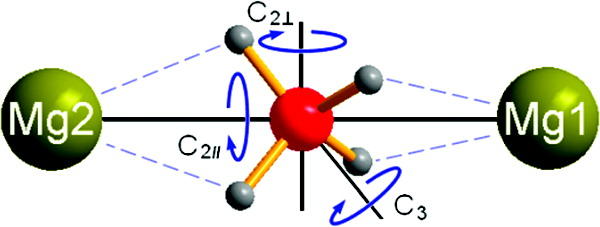
\includegraphics[width=0.5\linewidth]{mg-local-structure}
    \parbox{0.85\linewidth}{
\caption{%\footnote{Figure 9 from paper \ref{pap:magnesium}.}
Schematic representation of the environment of each \ce{B} atom, and how the different types of axes relates to it.
}
\label{fig:mg-local-structure}
}
\end{center}
\end{minipage}
\end{figure}

The experiments could not discern data for individual inequivelant sites but only averages for a given type of process.
Three distinct (average) processes were seen, all of which were for rotational diffusion.
Thus, the work exclusively revolved around understanding which rotations correpsonded with the experiments.

For each inequivelant site a number of rigid rotation PESes were constructed\footnote{Examples of which can be seen in figures 13 and 14 of paper \ref{pap:magnesium}} in order to get an overview of the interesting events and to limit computations spent on the costly MEP calculations, in a similar fashion as in \fref{sec:borohydrides-calcium}.
Due to symmetry not all the axes needed to be considered.

The general result from the PESes was that rotations that maximised the \ce{Mg}-\ce{H}, $d_{H-Mg}$ distance showed the lowest energies (\fref{fig:h-mg-distances}).
In this respect, two distinct types of $C_2$ axes were seen, those parallel to the \ce{Mg}-\ce{Mg} axis, $C_2^\parallel$, which maximised $d_{H-Mg}$ and those perpendicular to it, $C_2^\perp$, where $d_{H-Mg}$ was generally lower and showed higher barriers.
MEP calculations for $C_2^\perp$ found a combination of other axes yielded the same permutation but at a much lower energy cost.
The difference in relative barrier height decreased with decreasing $L$.\footnote{The relative difference would be non-existant for $L=0$ (and $L=\infty$) but non of the \ce{BH4} fulfill that critrion.}

\begin{figure}[h]
\begin{center}
  \subfigure[Average \ce{H}-\ce{Mg} distance]{
    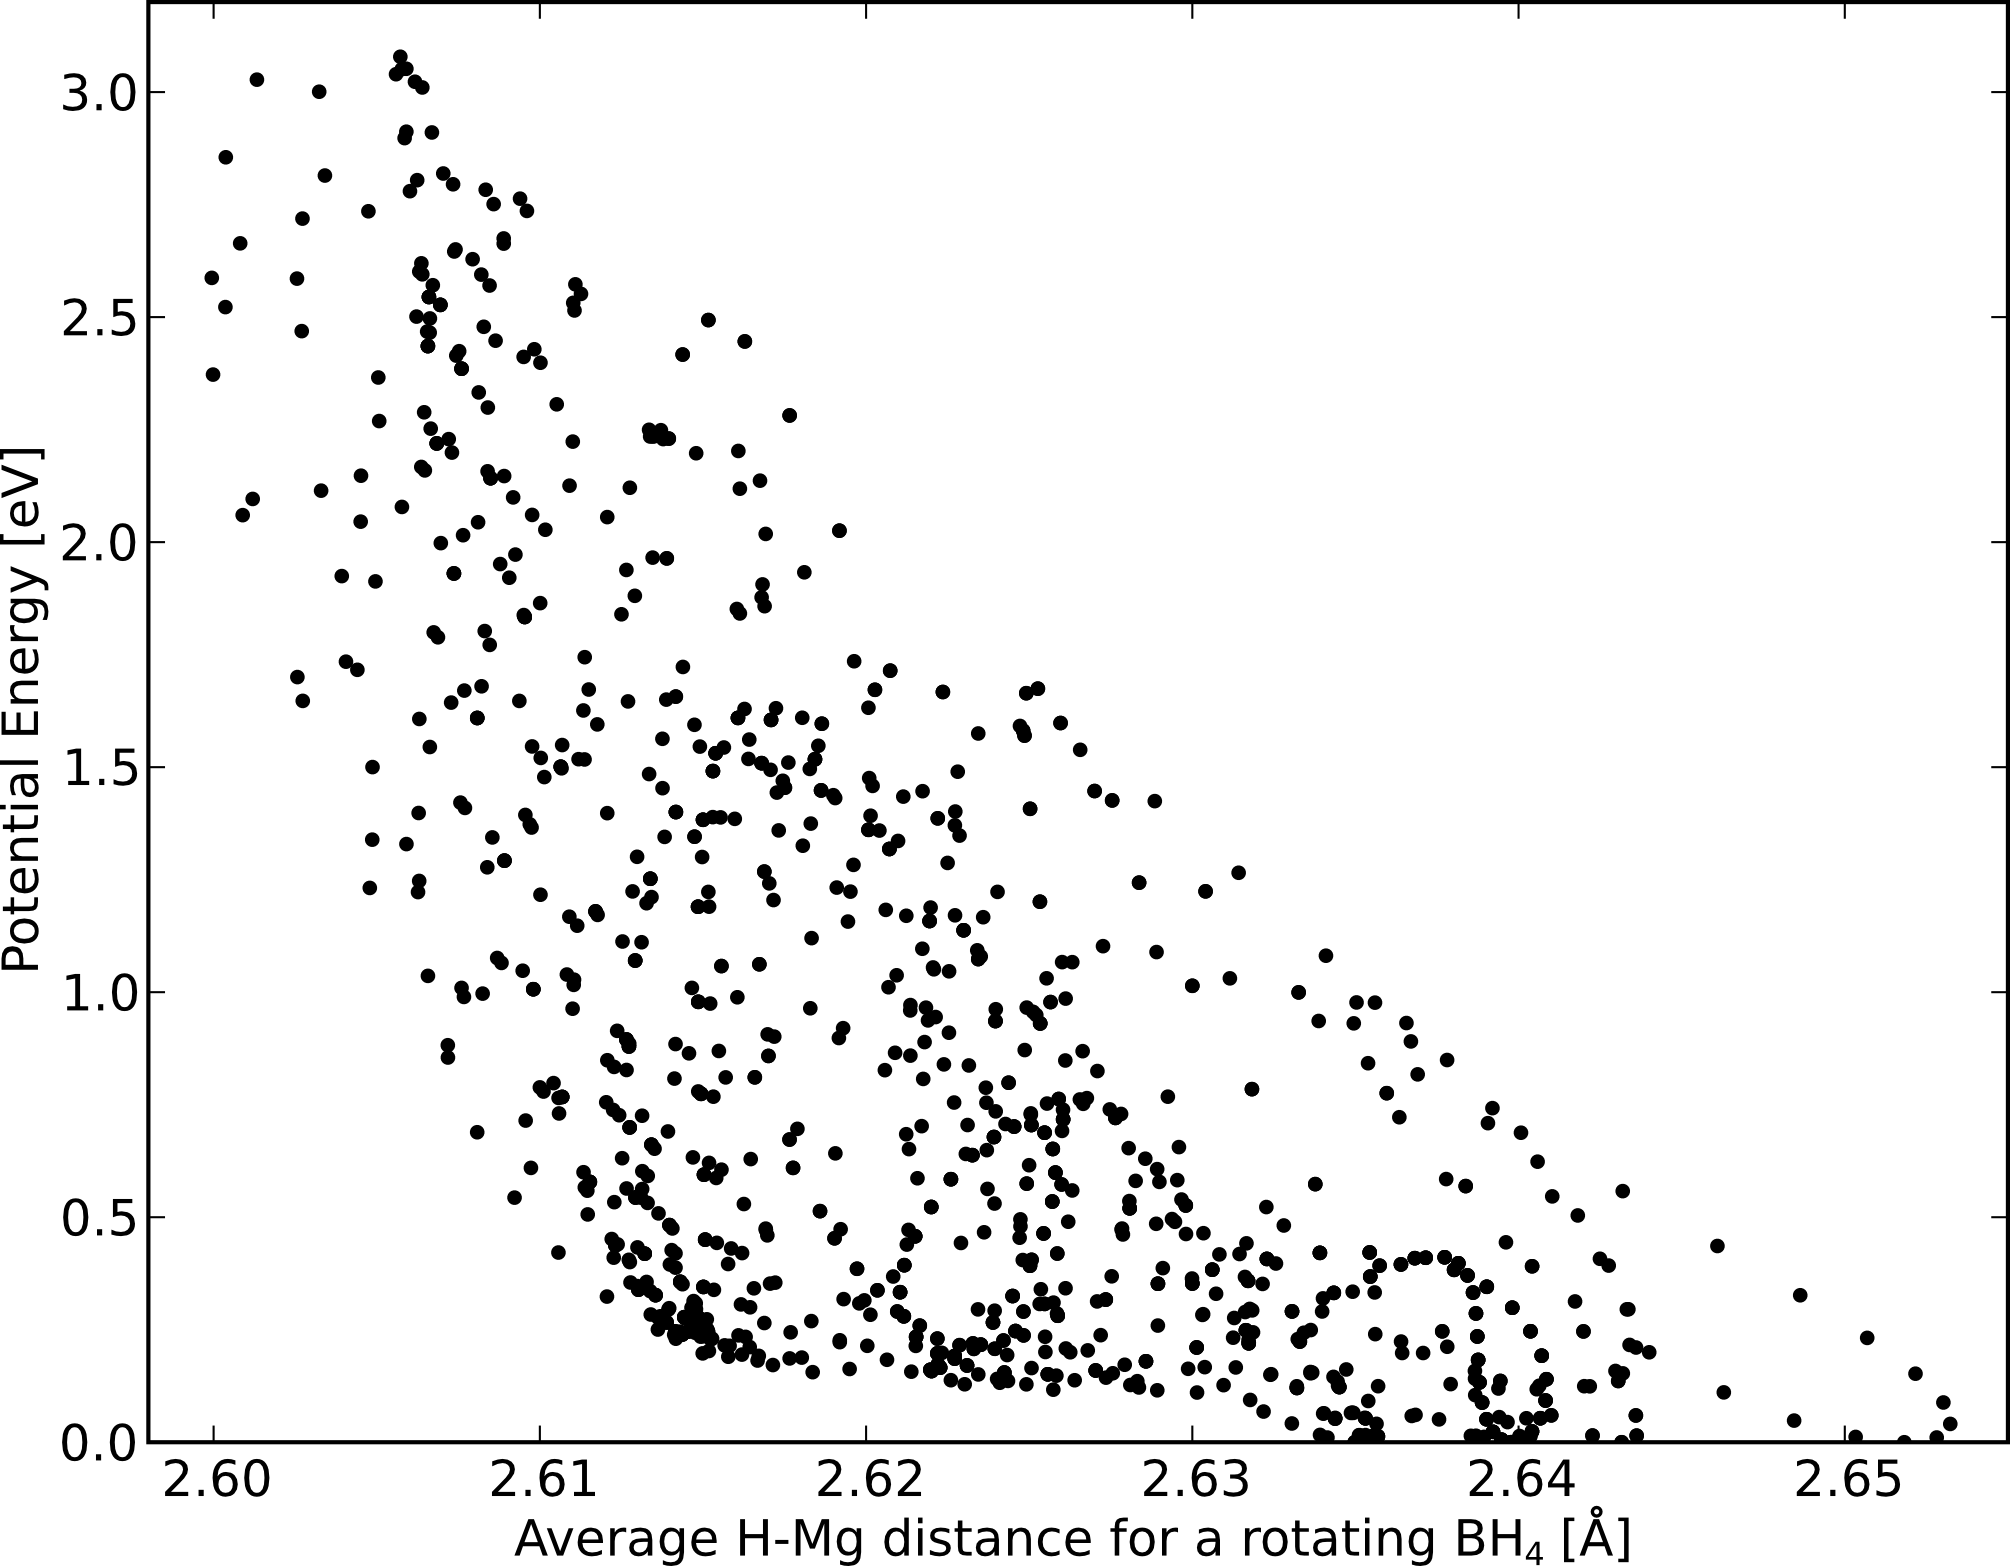
\includegraphics[width=0.45\linewidth]{h-mg-distances-avg}
    \label{fig:h-mg-distances-avg}
    }
  \subfigure[Minimum \ce{H}-\ce{Mg} distance]{
    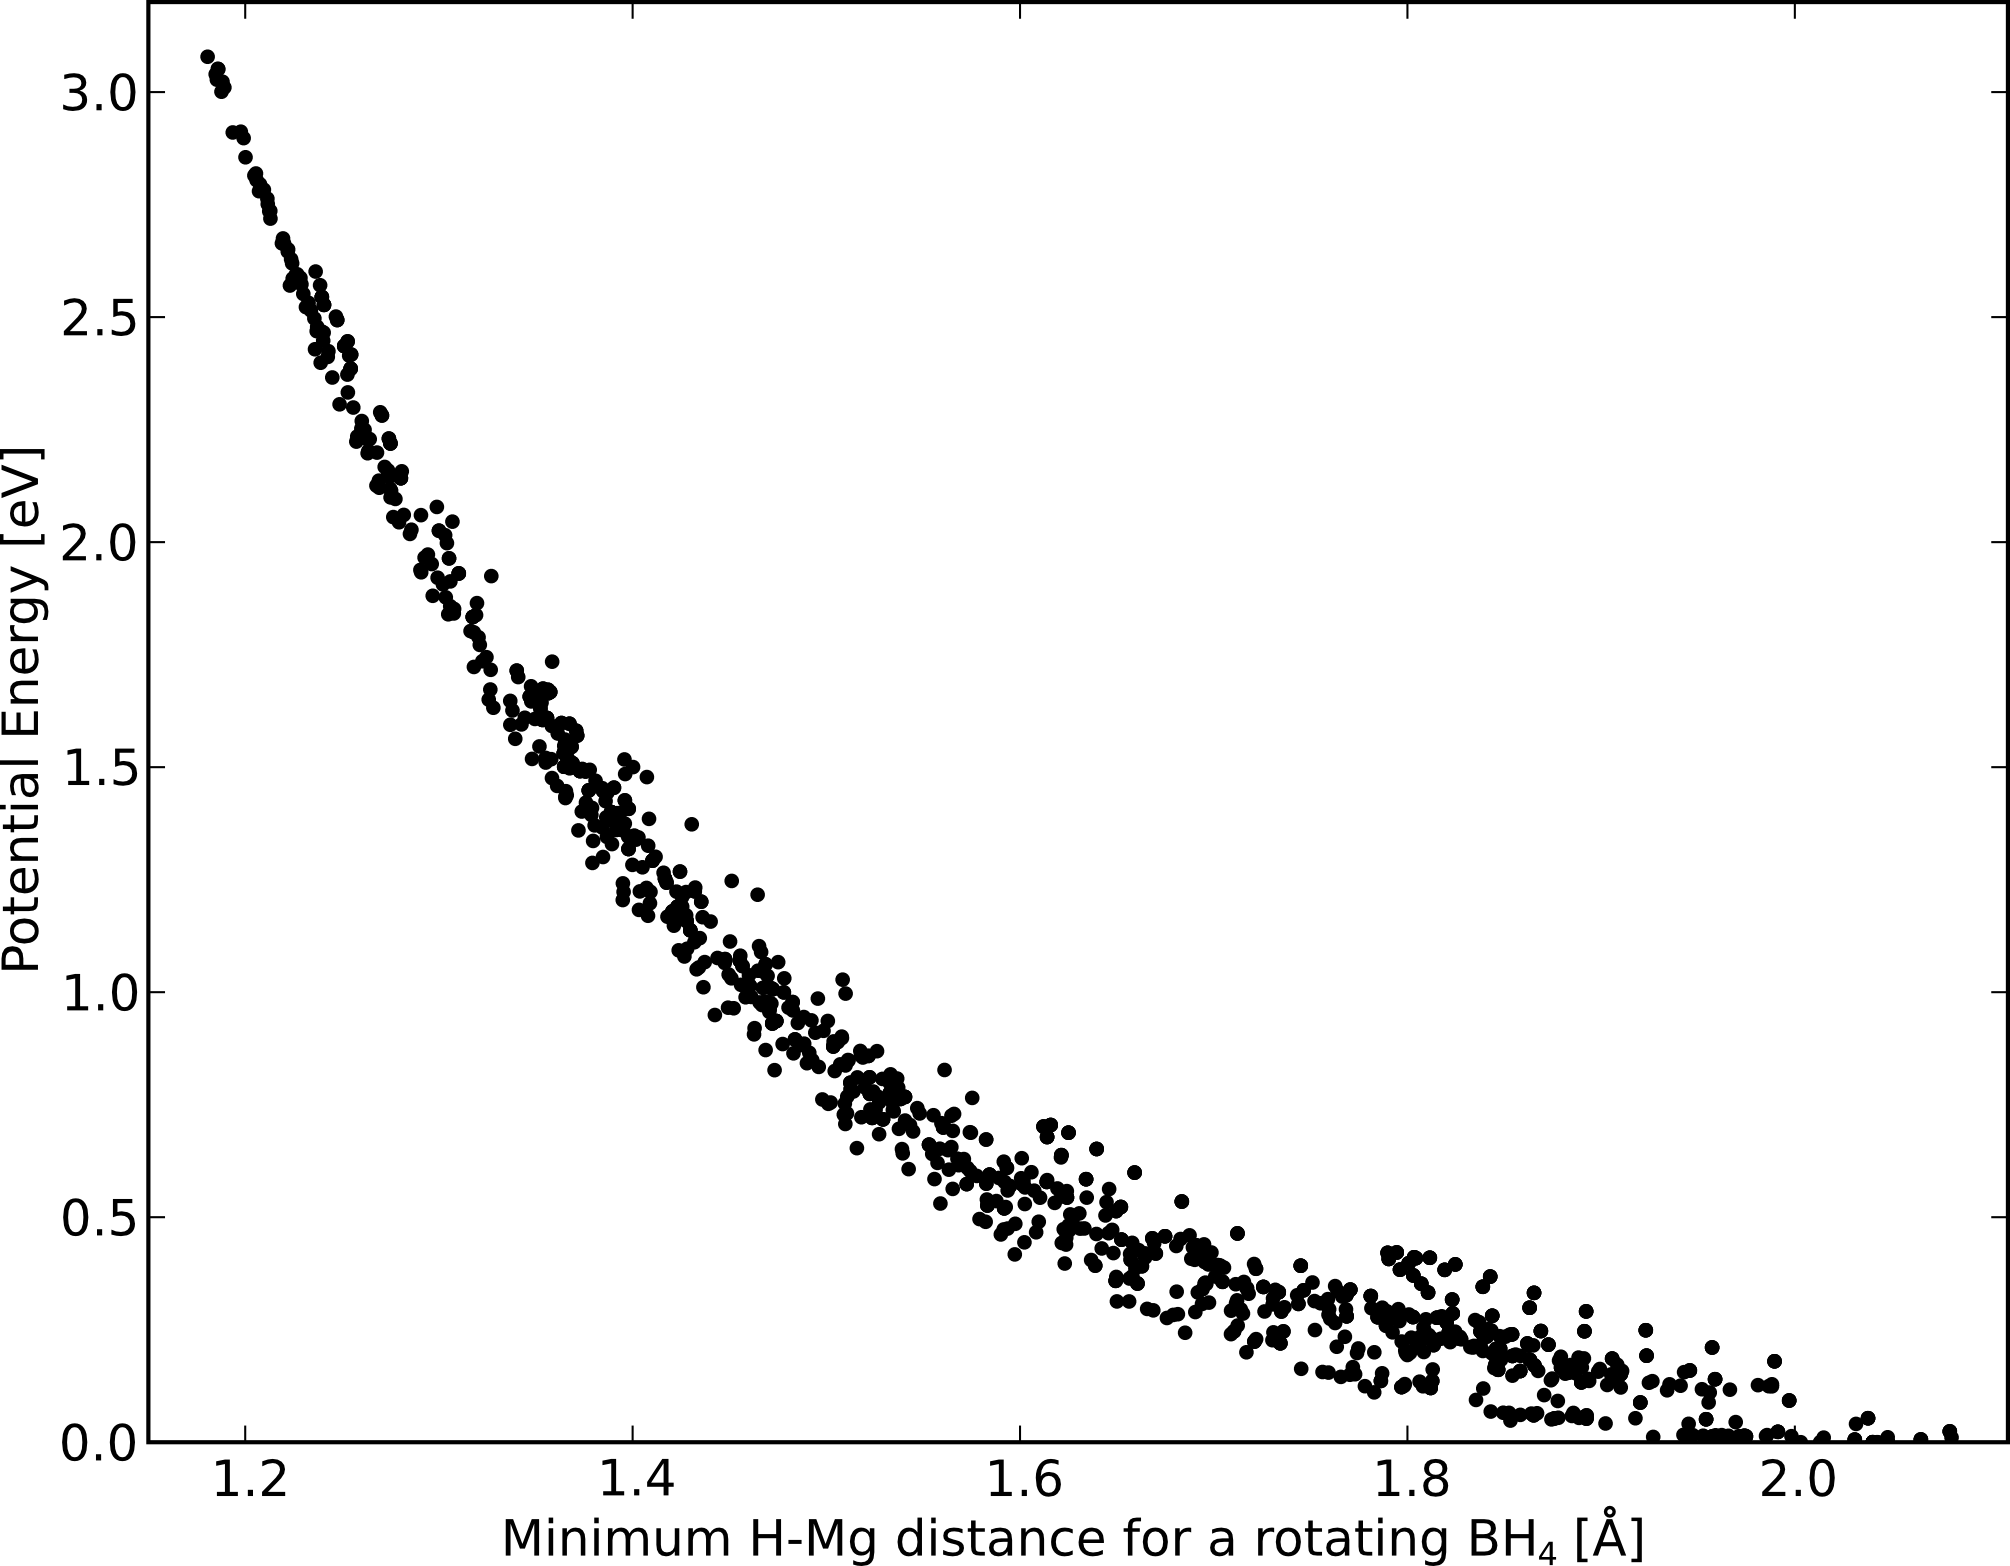
\includegraphics[width=0.45\linewidth]{h-mg-distances-min}
    \label{fig:h-mg-distances-min}
    }
    \parbox{0.85\linewidth}{
      \caption{For each PES, the distances between the \ce{H} atoms of the rotating \ce{BH4} unit to the neighboring \ce{Mg} atoms is plotted.
Some systematic features can be seen since the data was produced with specific rotations rather than a uniform distirubtion.
A clear trend for lower energies with higher distances can be seen.
      }
      \label{fig:h-mg-distances}
    }
\end{center}
\end{figure}

No such clear distinction could be made with regards to the $C_3$ axes.
However, due to symmetry many the $C_3$ axes for a given site yield a very similar PES and the rest would yield barriers that were not in any tune with the experimental results.

The rigid rotation plots are not able to give a full description of the events, neither their geometry nor their energetics.
Thus MEP calculations, for each symmetry inequivelant \ce{BH4}, were performed with the lowest energy rigid rotation paths as starting positions.

\begin{figure}[h]
\begin{center}
  \subfigure[The rotational energy barriers for \ce{BH4} in $\beta$-\ce{Mg(BH4)2}][%\footnotemark
The energy barriers as a function of $L$, the distance from the \ce{B} to the \ce{Mg}-\ce{Mg} axis.
The circles are the $C_2$ barriers, while the triangles are the $C_3$ axes.
A clear linear relationship (the line) can be seen for the $C_2$ axes.
]{
    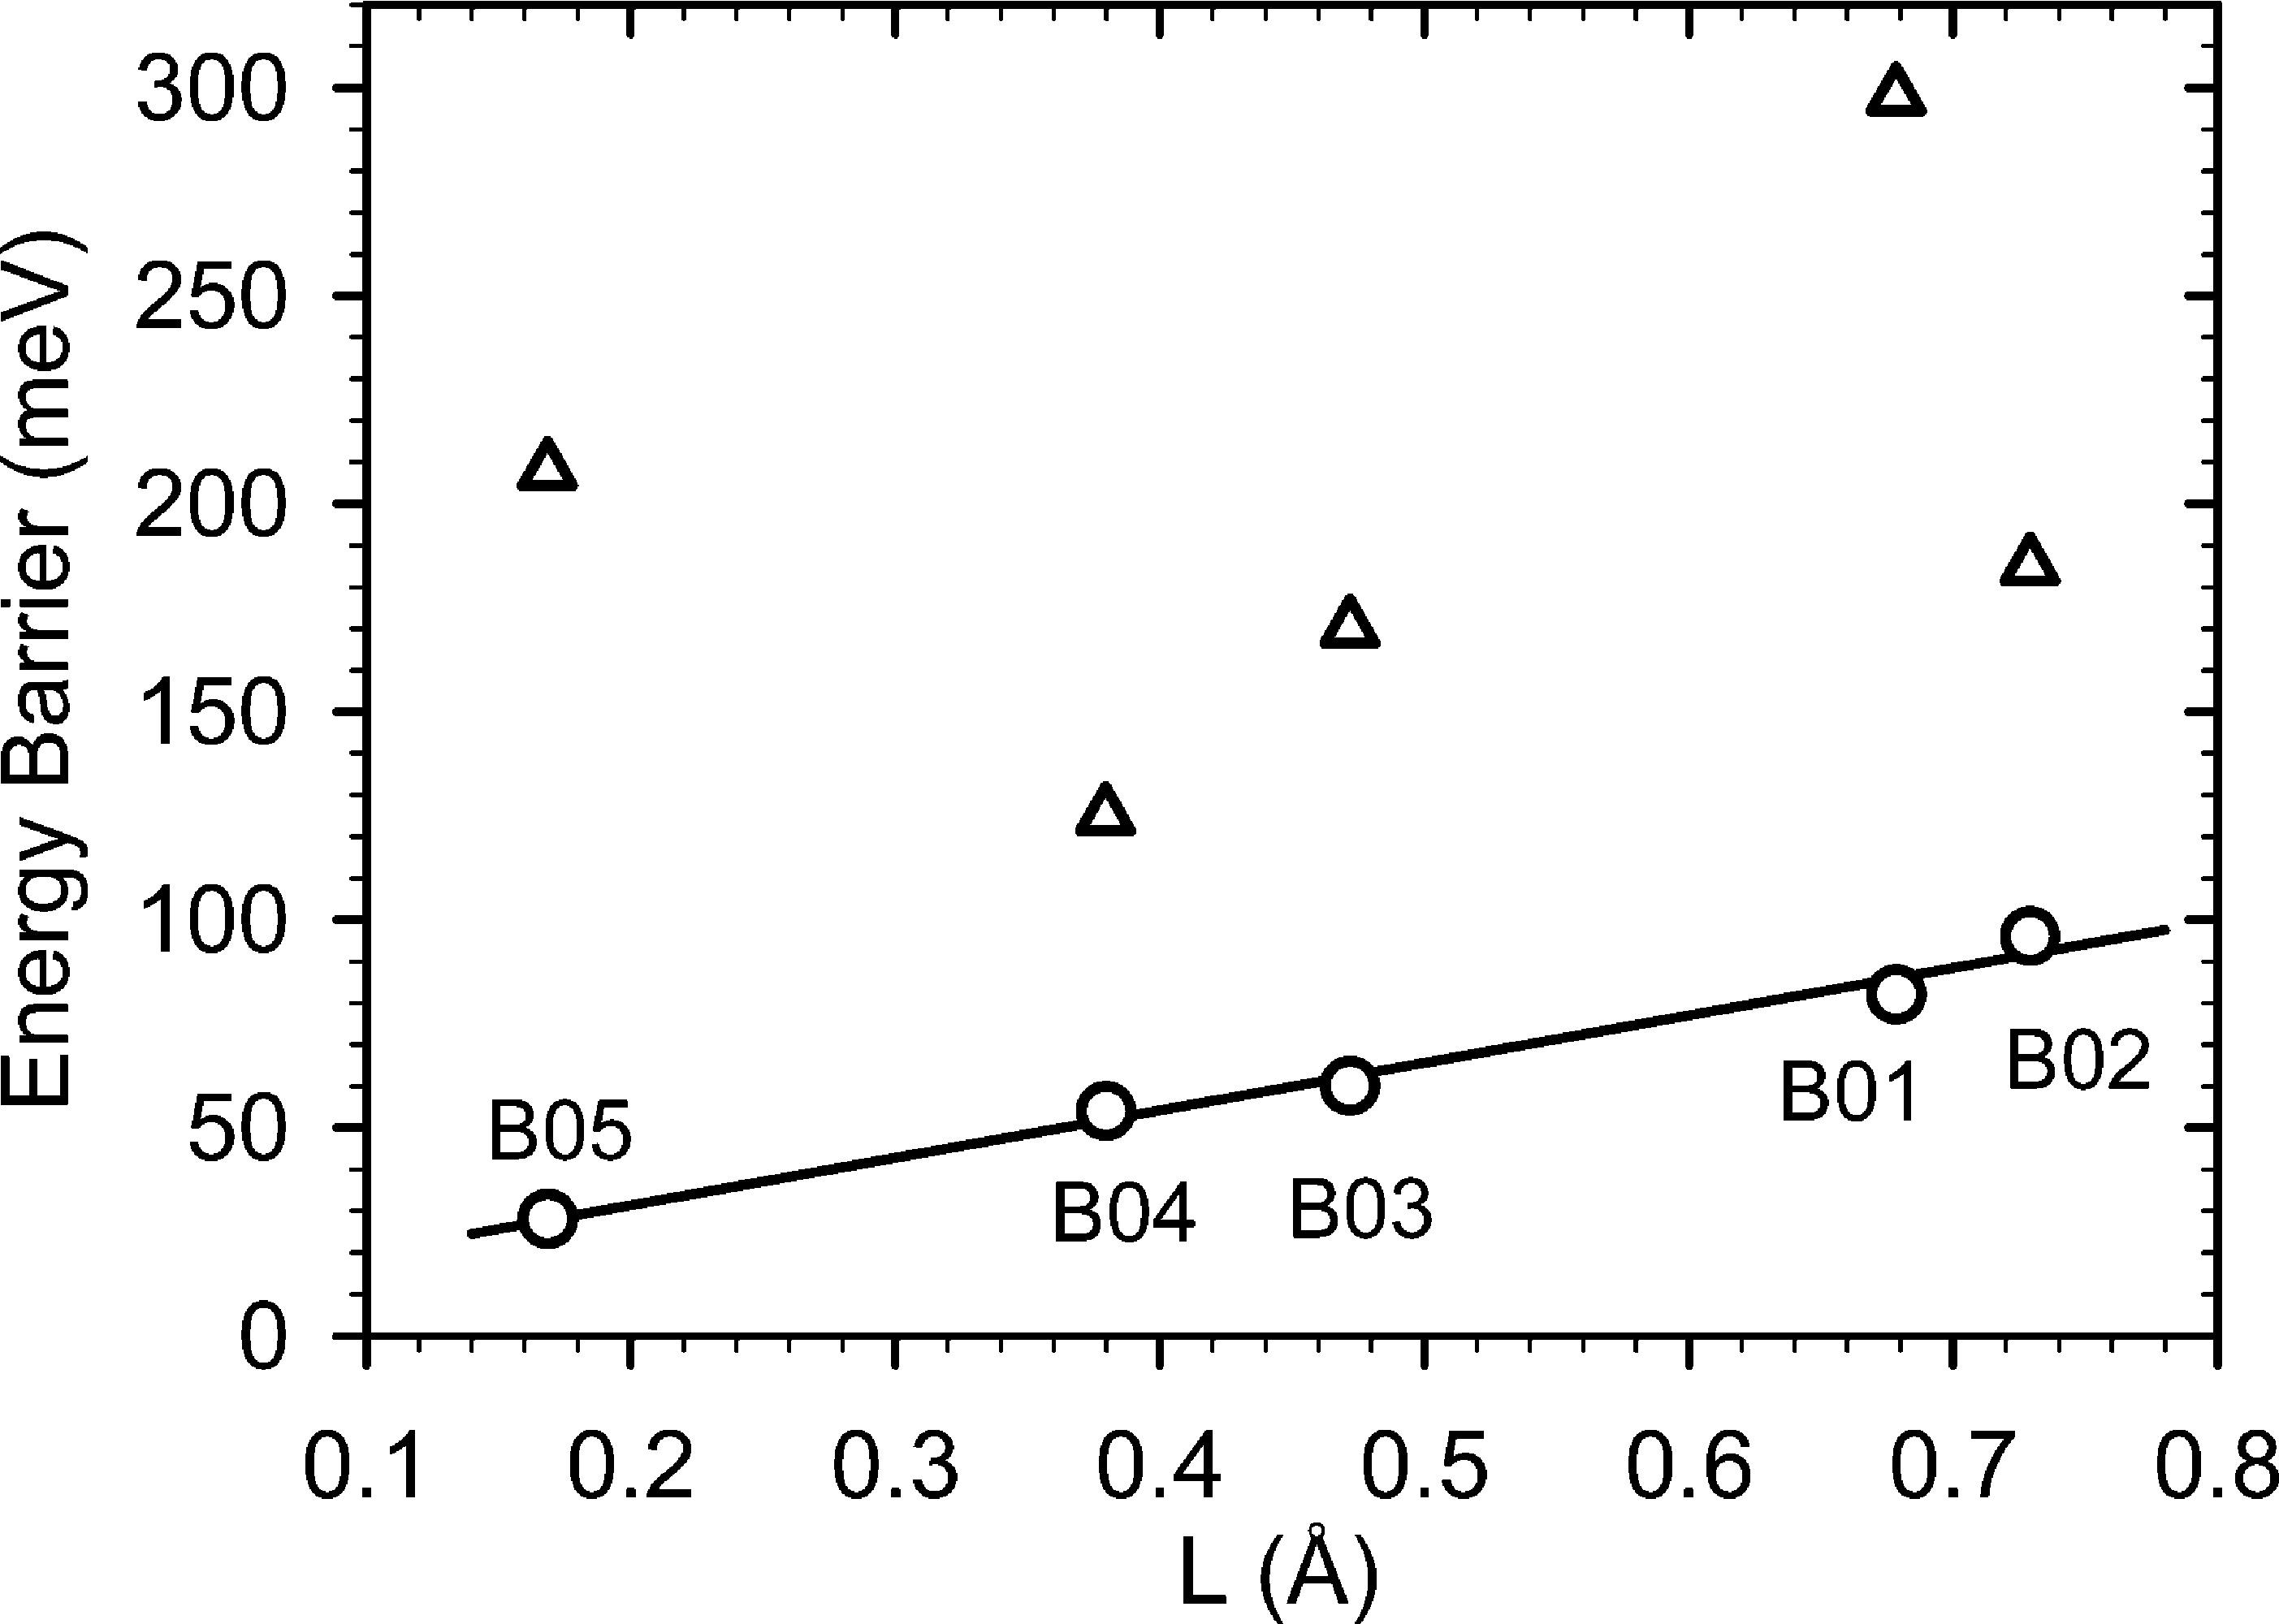
\includegraphics[width=0.45\linewidth]{mg-barriers}
    \label{fig:mg-barriers}
    }
  \subfigure[Comparison of the experimental and theoretical results][%\footnotemark
Comparison of the experimental and theoretical results.
Arrhenius-type behaviour, where $\Gamma = \Gamma_0 exp(-E_a / \kB T)$ and $\Gamma_0$ is the prefactor.
The circles, triangles and squares repesent the experimental data while the dashed and dash-dotted lines represent the theoretical data for the the $C_2^\parallel$ and $C_3$ type rotations, respectively.
  ]{
    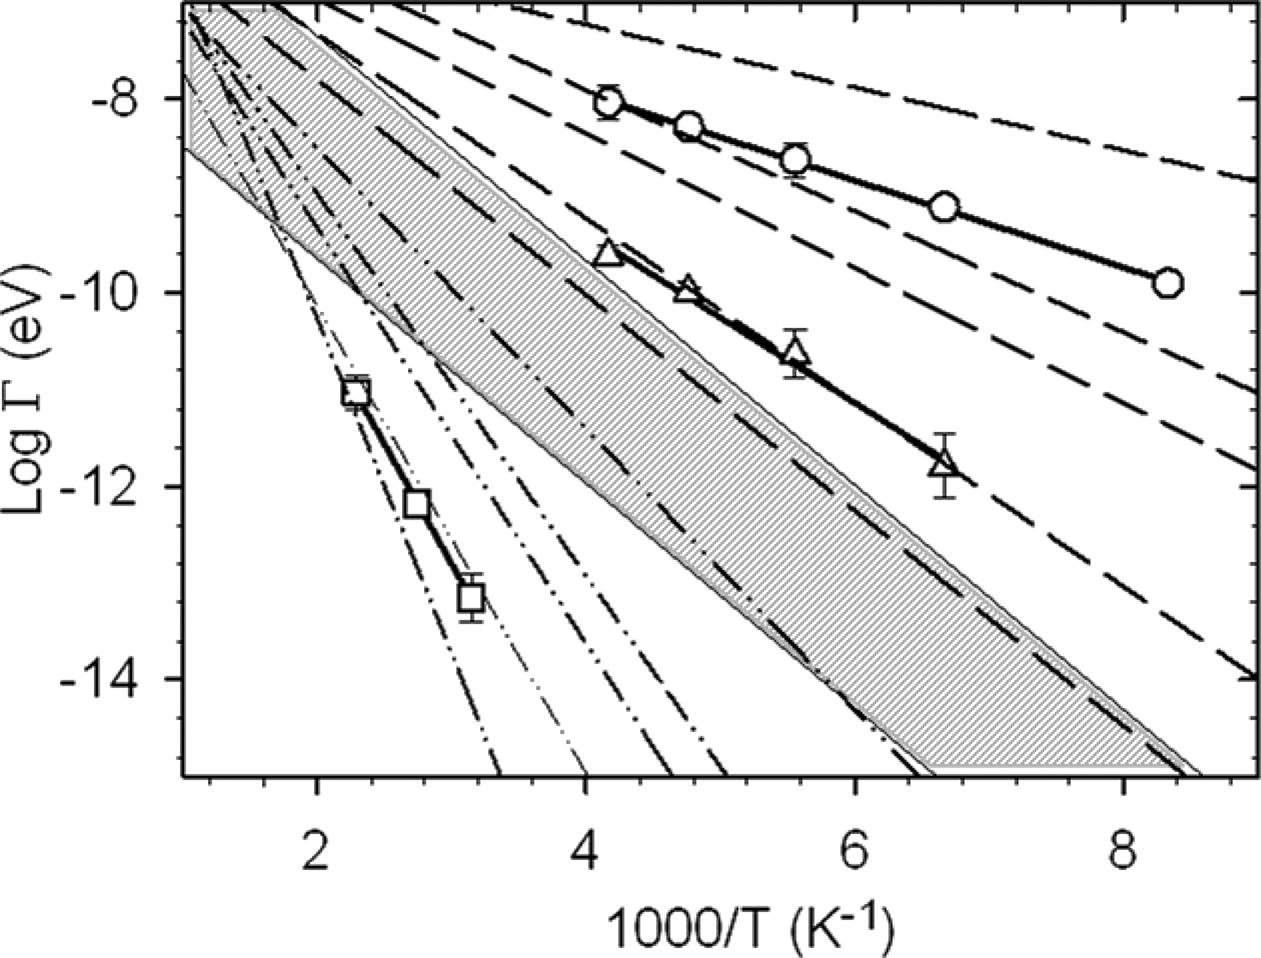
\includegraphics[width=0.45\linewidth]{mg-experimental-comparison}
    \label{fig:mg-experimental-comparison}
    }
\caption{The main results for $\beta$-\ce{Mg(BH4)2} 
\tred{Temporary graphics}
}
\label{fig:mg-results}
\end{center}
\end{figure}
%\footnotetext{Figure 17 from paper \ref{pap:magnesium}.}
%\footnotetext{Figure 11 from paper \ref{pap:magnesium}.}

It is unsurprising to find that there is, in fact, a direct relationship between $L$ and the $C_2^\parallel$ barrier height.
In fact, the relationship is linear, as can be seen in \fref{fig:mg-barriers}, the barrier increases with increased $L$ which is most likely due more \ce{H}-\ce{Mg} interaction.
Some of the $C_2$-type rotations showed a very shallow intermediate minimum ($\mytilde 4\times10^{-3} \unit{eV}$), associated with a slight stabilisation as $L$ decreased during the rotation.

On the other hand, no such direct relationship could be found for the $C_3$ axes, which were all found to be considerably higher in energy than the $C_2^\parallel$ axes.

\Fref{fig:mg-experimental-comparison} shows that the theoretical results (HTST reaction rates) form a distribution in which the experimental results fit rather well.
The $C_3$-type rotations 
The $C_2$-type rotations having a wider distribution and encompassing two of the experimental averages.


\expand


